%\documentclass{beamer}
\documentclass[handout]{beamer}
% This file is a solution template for:

% - Giving a talk on some subject.
% - The talk is between 15min and 45min long.
% - Style is ornate.

% Copyright 2004 by Till Tantau <tantau@users.sourceforge.net>.
%
% In principle, this file can be redistributed and/or modified under
% the terms of the GNU Public License, version 2.
%
% However, this file is supposed to be a template to be modified
% for your own needs. For this reason, if you use this file as a
% template and not specifically distribute it as part of a another
% package/program, I grant the extra permission to freely copy and
% modify this file as you see fit and even to delete this copyright
% notice. 

\mode<presentation>
{
  \usetheme{Montpellier}

  %\setbeamercovered{transparent}
  % or whatever (possibly just delete it)
}

\usepackage{xmpmulti} % package that defines \multiinclude

\usepackage[english]{babel}

\usepackage[latin1]{inputenc}

\usepackage{times}
\usepackage[T1]{fontenc}
% Or whatever. Note that the encoding and the font should match. If T1
% does not look nice, try deleting the line with the fontenc.

\title [Learning in repeated games] %(optional, use only with long paper titles)
{Online learning \\ in \\ repeated matrix games}

\author[Freund] % (optional, use only with lots of authors)
{Yoav Freund}
% - Give the names in the same order as the appear in the paper.
% - Use the \inst{?} command only if the authors have different
%   affiliation.

\institute[Universities of Somewhere and Elsewhere] % (optional, but mostly needed)

\subject{Machine Learning}
% This is only inserted into the PDF information catalog. Can be left
% out. 

% If you have a file called "university-logo-filename.xxx", where xxx
% is a graphic format that can be processed by latex or pdflatex,
% resp., then you can add a logo as follows:

% \pgfdeclareimage[height=0.5cm]{university-logo}{university-logo-filename}
% \logo{\pgfuseimage{university-logo}}



% Delete this, if you do not want the table of contents to pop up at
% the beginning of each subsection:
%% \AtBeginSubsection[]
%% {
%%   \begin{frame}<beamer>
%%     \frametitle{Outline}
%%     \tableofcontents[currentsection,currentsubsection]
%%   \end{frame}
%% }


% If you wish to uncover everything in a step-wise fashion, uncomment
% the following command: 

\beamerdefaultoverlayspecification{<+->}

\newcommand{\newmcommand}[2]{\newcommand{#1}{{\ifmmode {#2}\else\mbox{${#2}$}\fi}}}
\newcommand{\renewmcommand}[2]{\renewcommand{#1}{{\ifmmode {#2}\else\mbox{${#2}$}\fi}}}
\newcommand{\newmcommandi}[2]{\newcommand{#1}[1]{{\ifmmode {#2}\else\mbox{${#2}$}\fi}}}
\newcommand{\newmcommandii}[2]{\newcommand{#1}[2]{{\ifmmode {#2}\else\mbox{${#2}$}\fi}}}
\newcommand{\newmcommandiii}[2]{\newcommand{#1}[3]{{\ifmmode {#2}\else\mbox{${#2}$}\fi}}}

\newcommand{\algfnt}{\bf}

\newmcommand{\ouralg}{{\mbox{\algfnt Hedge}({\eta})}}

\newmcommand{\iter}{T}

\newfont{\cmmib}{cmmib10}
\newcommand{\boldell}{{\mbox{\cmmib \symbol{'140}}}}


\newmcommandi{\costvec}{{\boldell}_{#1}}
\newmcommandii{\cost}{{\ell}^{#1}_{#2}}

\newmcommandi{\rd}{\tilde{#1}}

\newmcommandi{\distvec}{{\bf p}^{#1}}
\newmcommandi{\rddistvec}{\rd{\bf p}^{#1}}
\newmcommandii{\dist}{{p}^{#1}_{#2}}
\newmcommandii{\rddist}{\rd{p}^{#1}_{#2}}

\newmcommandi{\bdistvec}{{\bf q}^{#1}}
\newmcommandii{\bdist}{{q}^{#1}_{#2}}

\newmcommandi{\wtvec}{{\bf w}^{#1}}
\newmcommandi{\rdwtvec}{\rd{\bf w}^{#1}}
\newmcommandii{\wt}{{w}^{#1}_{#2}}
\newmcommandii{\rdwt}{\rd{w}^{#1}_{#2}}


\newcommand{\Nweight}[2]{V_{#1}^{#2}}	%the normalized weight
\newcommand{\dweight}[2]{w^{#2}(#1)} % initial density measure
\newcommand{\TEloss}[1]{L_{#1}}	%total loss of expert i
\newcommand{\BEloss}{L_{\min}}	%total loss of the best expert
\newcommand{\TAloss}{L_A}	%total loss of algorithm
\newcommand{\weight}[2]{W_{#1}^{#2}} % weight assigned to expert
\newcommand{\btheta}{\hat{\theta}}

\newcommand{\R}[1]{{\color{red}{#1}}}
\newcommand{\B}[1]{{\color{blue}{#1}}}
\newcommand{\RM}[1]{{\color{red}{$#1$}}}


%BANDITS
\newcommand{\Aplay}{{\bf Hedge}}
\newcommand{\Aest}{{\bf Exp3}}
\newcommand{\Aesthp}{{\bf Exp3.P}}
\newcommand{\Aestg}{{\bf Exp3.P.1}}
\newcommand{\Aests}{{\bf Exp3.S}}
\newcommand{\Aessg}{{\bf Exp3.S.1}}
\newcommand{\Astrat}{{\bf Exp4}}
\newcommand{\Abound}{{\bf Exp3.1}}
\newcommand{\Gbest}{G_{\rm max}}

\newcommand{\defeq}{\stackrel{\rm def}{=}}
\newcommand{\compl}{\mbox{\sc h}}
\newcommand{\theset}[2]{\{ {#1} \,:\, {#2} \}}

\newmcommandii{\stratv}{\mbox{\boldmath $\xi$}^{#1}({#2})}

%Games paper
\newmcommand{\M}{\bf M}
\newmcommand{\dM}{\M'}
\newmcommand{\Row}{\bf R}
\newmcommand{\dRow}{\R'}
\newmcommand{\C}{\bf C}
\newmcommand{\dC}{\C'}
\newmcommand{\D}{D}
\renewmcommand{\P}{\bf P}
\newmcommand{\Q}{\bf Q}
\newmcommand{\Dt}{\D_t}
\newmcommand{\Pt}{\P_t}
\newmcommand{\Qt}{\Q_t}
\newmcommand{\Pstar}{\P^*}	% the min/max optimal mixed strategy
\newmcommand{\Pref}{\tilde{\P}}	% a reference mixed strategy (not
				% necessarily min/max)
\newmcommand{\Qstar}{\Q^*}
\newmcommand{\Pa}{\overline{\P}}
\newmcommand{\Qa}{\overline{\Q}}
\newmcommand{\Qh}{\hat{\Q}}
\newmcommandi{\trans}{{#1}^{\rm T}}
\newmcommand{\mhx}{\M(h,x)}
\newmcommand{\mxh}{\dM(x,h)}
\newmcommand{\mpq}{\M(\P,\Q)}
\newmcommand{\mpsq}{\M(\Pstar,\Q)}
\newmcommand{\mpsqt}{\M(\Pstar,\Qt)}
\newmcommand{\mptqt}{\M(\Pt,\Qt)}
\newmcommand{\mptt}{\M(\Pt,t)}
\newmcommand{\mptq}{\M(\Pt,\Q)}
\newmcommand{\mpqt}{\M(\P,\Qt)}
\newcommand{\minp}{\min_{\P}}
\newcommand{\maxq}{\max_{\Q}}
\newcommand{\RE}[2]{{\rm RE}\left( {#1} \; \parallel \; {#2} \right) }

\newmcommand{\sumt}{\sum_{t=1}^T}
\newmcommand{\sumin}{\sum_{i=1}^n}
\newmcommand{\delt}{\Delta_{T,n}}
\newcommand{\nextline}{\vspace{0.2cm}\\}   % a little space for equation arrays

\newcommand{\lwalg}{\mbox{\rm MW}}
\newcommand{\lwalgvar}{\mbox{\rm vMW}}

%%
\newcommand{\E}{\mbox{\rm\bf E}}
\newcommand{\p}[2]{p_{#1}(#2)}
\newcommand{\q}[2]{q_{#1}(#2)}
\newcommand{\x}[2]{x_{#1}({#2})}
\newmcommand{\bx}{\mbox{\boldmath$x$}}
\newmcommandi{\xv}{\bx({#1})}
\newmcommand{\xvt}{\xv{t}}
%\newcommand{\w}[2]{w_{#1}({#2})} replaced by \wt, but remember to switch order of parameters i and t
\renewcommand{\i}[1]{i_{#1}}
\newcommand{\hx}[2]{\hat{x}_{#1}(#2)}
\newcommand{\hxit}{\hx{\i{t}}{t}}
\newcommand{\pit}{\p{\i{t}}{t}}
\newcommand{\xit}{\x{\i{t}}{t}}
\newcommand{\expb}[1]{\exp\left(#1\right)}

\newcommand{\vp}{{\mathbf p}}
\newcommand{\vu}{{\mathbf u}}
\newcommand{\vv}{{\mathbf v}}
\newcommand{\vx}{{\mathbf x}}
\newcommand{\vy}{{\mathbf y}}
\newcommand{\vw}{{\mathbf w}}
\newcommand{\vq}{{\mathbf q}}

\newcommand{\vecq}{{\bf q}}
\newcommand{\vecp}{{\bf p}}


\newcommand{\HedgeLoss}{L_{\mbox{\footnotesize Hedge}}}

\newcommand{\W}{\vec{W}}
\newcommand{\V}{\vec{V}}
\newcommand{\X}{\vec{X}}
\newcommand{\vb}{\vec{b}}
%\newcommand{\loss}{\vec{\ell}}
\newcommand{\loss}{L}
\newcommand{\elloss}[2]{\ell_{#2}\left( #1 \right)} %loss of expert i at time t
\newcommand{\lossvec}[1]{{\mathbf \ell}_{#1}}       %loss of expert at time t
\newcommand{\w}[1]{\makebox[12pt]{{#1}}}
\newcommand{\Rps}{\mbox{\tt R}}
\newcommand{\rPs}{\mbox{\tt P}}
\newcommand{\rpS}{\mbox{\tt S}}
\newcommand{\rpstie}{\w{$\frac{1}{2}$}}
\newcommand{\rpswin}{\w{$0$}}
\newcommand{\rpsloss}{\w{$1$}}

\newmcommand{\decspace}{\Delta}
\newmcommand{\decsym}{\delta}
\newmcommandi{\dec}{\decsym^{#1}}
\newmcommand{\decdistsym}{\cal D}
\newmcommandi{\decdist}{{\decdistsym}^{#1}}

\newmcommand{\simpdistspace}{{\bf \cal S}}
\newmcommand{\domset}{{\rm dom}(\decdistsym)}

\newmcommand{\expdistsym}{{\cal E}}
\newmcommandii{\expdist}{{\expdistsym}^{#1}_{#2}}
\newmcommand{\expdecsym}{{\varepsilon}}
\newmcommandii{\expdec}{\expdecsym^{#1}_{#2}}

\newmcommand{\outspace}{\Omega}
\newmcommand{\outsym}{\omega}
\newmcommandi{\out}{\outsym^{#1}}

%\newmcommandii{\Dkl}{D_{\mbox{kl}}\paren{#1||#2}}
\newmcommandii{\Dkl}{{\rm {KL}}\paren{{#1}\;||\;{#2}}}

\newmcommandi{\sumwts}{\sum_{i=1}^N \wt{#1}{i}}

\newmcommand{\lossalg}{L_A}
\newmcommand{\lossouralg}{{L_{\mbox{\scriptsize\algfnt Hedge}(\eta)}}}
\newmcommand{\lossS}{{L_{\mbox{\scriptsize\algfnt S}}}}
\newmcommandi{\lossi}{L_{#1}}
\newmcommandii{\lossit}{L_{#1}^{#2}}

\newmcommandi{\upbnd}{\tilde{#1}}

\newcommand{\angles}[1]{{\left\langle {#1} \right\rangle}}
\newcommand{\paren}[1]{{\left( {#1} \right)}}
\newcommand{\brac}[1]{{\left[ {#1} \right]}}
\newcommand{\braces}[1]{{\left\{ {#1} \right\}}}

\newcommand{\abs}[1]{{\left| {#1} \right|}}
\newcommand{\ceiling}[1]{{\left\lceil {#1} \right\rceil}}

\newfont{\msym}{msbm10}
\newcommand{\real}{\mbox{\msym R}}

\newmcommand{\updatefcn}{U_\eta}

%% \newtheorem{theorem}{Theorem}	
%% \newtheorem{lemma}[theorem]{Lemma}
%% \newtheorem{corollary}[theorem]{Corollary}
%% \newtheorem{definition}{Definition}

%\newcommand{\proof}{\noindent{\bf Proof:} }
%\newcommand{\example}[1]{{\em Example #1.} }
%\newcommand{\qed}{\rule{0.7em}{0.7em}}

\newcommand{\WeakAlg}{\mbox{\algfnt WeakLearn}}
\newcommand{\Boost}{\mbox{\algfnt AdaBoost}}
\newcommand{\EX}{\mbox{\bf EX}}
\newmcommand{\hf}{h_{{f}}}
\newmcommand{\rdhf}{\rd{h}_{{f}}}
\newmcommand{\hfT}{h^T_{{f}}}
\newmcommand{\ranh}{{b}}

\newmcommand{\conclass}{{\cal C}}

\newmcommand{\badvec}{{\bf b}}
\newmcommandi{\bad}{{b}_{#1}}

%%%%%%%% New commands defined for the game-playing paper

\newmcommand{\hedge}{\algfnt Hedge}
\newmcommand{\play}{\algfnt Play}
\newmcommandi{\Glossvec}{{\bg y}^{#1}}
\newmcommandii{\Gloss}{{y}^{#1}_{#2}}
%\newmcommandi{\action}{{I}_{#1}}
\newmcommandi{\Gdistvec}{{\bf \tilde{p}}^{#1}}
\newmcommandii{\Gdist}{{\teilde{p}}^{#1}_{#2}}

%%%%%%%%%%%%%%%%%%%%%%%%%%%%%%%%%%%%%%%%%%%%%%%%%%%%%
\newmcommand{\Idistvec}{{D}}
\newmcommandi{\Idist}{\Idistvec({#1})}
\newmcommand{\Idistt}{\Idistvec_t}

\newmcommand{\Xdist}{{\cal P}}
\newmcommand{\emp}{\hat{\epsilon}}

\newmcommand{\classpc}{Y}
\newmcommand{\numclass}{k}
\newmcommandii{\prob}{\mbox{\rm Pr}_{#1}\left[{#2}\right]}
\newmcommandii{\exval}{\mbox{\rm E}_{#1}\left[{#2}\right]}

%\usepackage{amsmath}
\DeclareMathOperator*{\argmax}{argmax} % thin space, limits underneath in displays
\DeclareMathOperator*{\argmin}{argmin} 

\newcommand{\RR}{\mathbb{R}}
\newcommand{\regret}{\mbox{Regret}}

%%% Conditional probabilities
\newmcommandii{\condp}{p\left( #1 \left| #2 \right. \right)}

\newmcommand{\lab}{y}
\newmcommand{\ploss}{\mbox{ploss}}
\newmcommandii{\avploss}{\ploss_{#1}({#2})}
\newcommand{\sfrac}[2]{\mbox{$\frac{#1}{#2}$}}

\newcommand{\mboosta}{\mbox{\algfnt AdaBoost.M1}}
\newcommand{\mboostb}{\mbox{\algfnt AdaBoost.M2}}
\newcommand{\mboostr}{\mbox{\algfnt AdaBoost.R}}

%\newmcommand{\slos}{\mbox{ploss}}
%\newmcommandiii{\sloss}{\slos_{#1}({#2},{#3})}
%\newmcommandiii{\avsloss}{\slos_{{#1},{#2}}({#3})}

\newmcommandii{\vwt}{{W}^{#1}_{#2}}

\newcommand{\figline}{\rule{\textwidth}{1pt}}

%\newmcommandi{\1}{{\bf 1}({#1})}
\newmcommandi{\1}{[\![{#1}]\!]}

\newmcommand{\confcn}{\kappa}
\newmcommandi{\erint}{\abs{\int_{y_i}^{h_t(x_i)} {#1} dy}}
%\newmcommandi{\erint}{\int_{\min\{y_i,h_t(x_i)\}}^{\max\{y_i,h_t(x_i)\}}{#1}dy}


\begin{document}

\begin{frame}
  \titlepage
Based on ``Adaptive Game Playing Using Multiplicative Weights'' Freund
and Schapire.
\end{frame}

\begin{frame}
  \frametitle{Outline}
  \tableofcontents[pausesections]
  % You might wish to add the option [pausesections]
\end{frame}

\section{Repeated Matrix Games}

\begin{frame}
\frametitle{Zero sum games in matrix form}
\begin{itemize}
\item Game between two players.
\item Defined by \R{$n \times m$} matrix \R{$\M$}
\item \B{Row} player chooses \R{$i \in \{1,\ldots,n\}$}
\item \B{Column} player chooses \R{$j \in \{1,\ldots,m\}$}
\item \B{Row} player gains \R{$\M(i,j) \in [0,1]$}
\item \B{Column} player looses \R{$\M(i,j)$}
\item Game repeated many times.
\end{itemize}
\end{frame}

\begin{frame}
  \frametitle{Pure vs. mixed strategies}
  \begin{itemize}
  \item Choosing a \B{single} action = \B{pure} strategy.
  \item Choosing a \B{Distribution} over actions = \B{mixed} strategy.
  \item \B{Row} player chooses dist. over rows \R{$\P$}
  \item \B{Column} player chooses dist. over columns \R{$\Q$}
  \item \B{Row} player gains \R{$\M(\P,\Q)$}.
  \item \B{Column} player looses \R{$\M(\P,\Q)$}.
  \end{itemize}
\end{frame}

\begin{frame}
  \frametitle{Mixed strategies in matrix notation}
  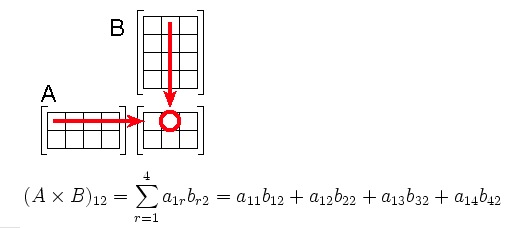
\includegraphics[width=8cm]{figures/matrixProduct.jpg}
\begin{itemize}
\item  \R{$\Q$} is a \B{column} vector. \R{$\P^T$} is a row vector.
\item  \R{$\M(\P,\Q) = \P^T \M \Q = \sum_{i=1}^n \sum_{j=1}^m \P(i)
    \M(i,j) \Q(j)$}
  \end{itemize}
\end{frame}

\begin{frame}
  \frametitle{The minmax Theorem}
~\\
When using pure strategies, second player has an advantage.
~\\~\\ ~\pause
\B{John von Neumann, 1928.}
\\ ~ \\ 
\R{\[ \minp \maxq \mpq = \maxq \minp \mpq \]}
\\ ~ \\ 
In words:
\begin{itemize}
  \item for \B{pure} strategies, choosing second can be better.
  \item for \B{mixed} strategies, choosing second gives no advantage.
  \item There are min-max optimal mixed Strategies: \R{$\P^*,\Q^*$}
  \item \R{$M(\P^*,\Q^*)$} is the \B{value} of the game.
\end{itemize}
\end{frame}


\section{Specific games}

\begin{frame}
\frametitle{Online Learning as matrix game}
  \begin{itemize}
  \item Row = action
  \item Column = iteration.
  \item Player chooses mixed strategy \R{$\P_t$}
  \item adversary chooses pure strategy \R{$\Q_t = \langle 0,\cdots,0,1,0,
      \cdots, 0\rangle$} the \R{$1$} is at position \R{$t$}
%  \item Loss: \R{$L_T = \sum_{t=1}^T \M(\P_t,\Q_t)$}
  \item Goal  - minimize regret: \R{$\sum_{t=1}^T \M(\P_t,\Q_t) -
      \sum_{t=1}^T \M(\P^*,\Q_t)$}
  \end{itemize}
\[  \begin{array}{l|c|c|c}
      & t=1 & t=2 & \ldots  \\
      \hline
    expert 1 & 0    & 1 & \ldots\\
    expert 2 & 0.2    & 0.1  & \ldots\\
    expert 3 & 0.5    & 0.2  & \ldots\\
      \ldots & \ldots    & \ldots  & \ldots\\
      \hline
    Master & 0.35 & 0.13 & \ldots 
    \end{array}
\]
\end{frame}

\begin{frame}
\frametitle{Boosting as a matrix game (1)}
  \begin{itemize}
  \item Row = example \R{$(x,y)$}
  \item Column = Weak Rule \R{$h_t$}
  \item Matrix entry for \R{$(x,y),h_t$} is \R{$0$} if \R{$h_t(x)=y$},
    \R{$1$} \R{$h_t(x) \neq y$}
\end{itemize}
\[  \begin{array}{l|c|c|c}
      & h_1 & h_2 & \ldots  \\
      \hline
    example 1 & 0    & 1 & \ldots\\
    example 2 & 1    & 0  & \ldots\\
    example 3 & 0    & 0  & \ldots\\
      \ldots & \ldots    & \ldots  & \ldots\\
      \hline
    \end{array}
  \]
\end{frame}

\begin{frame}
  \frametitle{Boosting as a matrix game (2)}
  \begin{itemize}
\item Boosting assumption: for any distribution over examples, there
    exists a weak rule with weighted error \R{$<1/2$}
  \item In game terms: For any \B{mixed strategy} of the row player \R{$\P$},
    there is a \B{pure strategy} for column player \R{$\Q = \langle 0,\cdots,0,1,0,
      \cdots, 0\rangle$} such that \R{$M(\P,\Q)<1/2$)}
  \item From Min-Max theorem: There exists a column mixed strategy (a
    distribution over weak rules), that has expected value larger than
    zero for any row pure strategy ( = any example).
  \item The weighted majority vote over the weak rule is \B{\bf always} correct. 
\end{itemize}
\end{frame}

\begin{frame}
\frametitle{Adaboost as a repeated matrix game}
\begin{itemize}
\item Booster chooses distribution over examples = mixed strategy
  over rows \R{$\P_t$}
\item adversary chooses weak rule \R{$\Q_t = \langle 0,\cdots,0,1,0,
    \cdots, 0\rangle$} the \R{$1$} is at position \R{$t$}
  % \item Loss: \R{$L_T = \sum_{t=1}^T \M(\P_t,\Q_t)$}
\item \B{\bf Goal 1:} produce a weighted majority rule that is highly
  accurate.
\item \B{\bf Goal 2:} Find a \B{``hard''} distribution over the training examples.
\end{itemize}
\[  \begin{array}{l|c|c|c}
      & h_1 & h_2 & \ldots  \\
      \hline
      example 1 & 0    & 1 & \ldots\\
      example 2 & 1    & 0  & \ldots\\
      example 3 & 0    & 0  & \ldots\\
      \ldots & \ldots    & \ldots  & \ldots \\
                                     \hline
    \end{array}
  \]
\end{frame}



\section{Minmax vs. Regret}

\begin{frame}
\frametitle{Minmax is weaker than diminishing regret}
\begin{itemize}
\item The minmax theorem proves the existence of an \B{Equilibrium}.
\item Learning guarantees no regret with respect to the past.
\item If all sides use learning, then game will converge to minmax equilibrium.
\item If opponent is not optimally adversarial (limited by knowledge, computationa power...) then learning gives \B{better} performance than min-max.
\item Our goal is to minimize regret.
\end{itemize}
\end{frame}

\section{Fictitious play}

\begin{frame}
\frametitle{Fictitious play}
\begin{itemize}
\item also called \B{``Follow the leader''}
\item Choose the best action with respect to the sum of past loss vectors.
\item Might not converge to optimal mixed strategy.
\item Consider playing the matching coins game against an adversary
  that alternates \B{HTHTHTHTHT}
\item If \#H > \#T the next element is T
\item If \#T > \#H the next element is H
\item follow the leader makes an error on each iteration.
\end{itemize}
\end{frame}

\begin{frame}
\frametitle{Randomized Fictitious play}
\begin{itemize}
\item Also called \B{'Follow the perturbed leader'}
\item Choose the best action with respect to the sum of past loss
  vectors \R{plus noise}.
\item Adding noise allows us to choose responses that are slightly
  worse than best response.
\item \B{Hannan 1957} Randomized ficticus play converges to regret
  minimizing strategy.
  \item regret is \R{$O(1/\sqrt{n})$} where \R{$n$} is number of actions.
\end{itemize}
\end{frame}


\section{Strategy using Hedge}

\begin{frame}
\frametitle{The basic algorithm}
\begin{itemize}
\item Choose an initial distribution \R{$\P_1$}
\item \R{$$\P_{t+1}(i) = \P_{t}(i) {e^{-\eta \M(i,\Qt)} \over Z_t}$$}
\item Where \R{$Z_t = \sum_{i=1}^n \P_{t}(i) e^{-\eta \M(i,\Qt)}$}
\item \R{$\eta>0$} is the learning rate.
\end{itemize}
\end{frame}


\section{The basic analysis}

\begin{frame}
  \frametitle{Generalized regret bound}
  \begin{itemize}
  \item Regret relative to the best {\em pure strategy}
    \R{$i$}
    \R{\small{\[
          \sumt \mptqt \leq \paren{\frac{1}{1-e^{-\eta}}}\;
          \min_i \brac{\eta\; \sumt \M(i,\Qt) - \ln \P_1(i)}
        \]}}
  \item    regret with respect the the best {\em mixed strategy}
    \R{$\P$}:
    \R{\small{\[
          \sumt \mptqt \leq \paren{\frac{1}{1-e^{-\eta}}}\;
          \minp \brac{\eta\; \sumt \mpqt + \RE{\P}{\P_1}}
        \]}}
  \item \small{Where \R{$$ \RE{\P}{\Q}\doteq \sum_{i=1}^n \P(i) \ln \frac{\P(i)}{\Q(i)}$$}}
  \end{itemize}
\end{frame}

\begin{frame}
\frametitle{Main Theorem}
\begin{itemize}
\item For \B{any} game matrix $\M$.
\item Any sequence of mixed strat. \R{$\Q_1,\ldots,\Q_T$}
\item The sequence \R{$\P_1,\ldots,\P_T$} produced by \\
basic alg using \R{$\eta>0$} satisfies
\R{\[
   \sumt \mptqt \leq \paren{\frac{1}{1-e^{-\eta}}}\;
        \minp \brac{\eta\; \sumt \mpqt + \RE{\P}{\P_1}}
\]}
\end{itemize}
\end{frame}


\begin{frame}
\frametitle{Corollary}
\begin{itemize}
\item Setting \R{$ \eta = \ln \paren{ 1+\sqrt{\frac{2\ln n}{T}} }$}
\item the average per-trial loss is
\R{\[
   \frac{1}{T} \sumt \mptqt \leq
    \minp \frac{1}{T} \sumt \mpqt + \delt
\]}
\item Where 
\R{\[
\delt = \sqrt{2 \ln n \over T} + {\ln n \over T} 
= O\paren{\sqrt{\frac{\ln n}{T}}}.
\]}
\end{itemize}
\end{frame}

% \iffalse
% \begin{frame}
% \frametitle{Main Lemma}

% On any iteration \R{$t$}
% \\ ~ \\ \pause
% For any mixed strategy \R{$\Pref$}
% \\ ~ \\ \pause
% \R{$
% \RE{\Pref}{\P_{t+1}} - \RE{\Pref}{\P_t} \leq 
% \eta \M(\Pref,\Q_t)  - (1-e^{-\eta})\M(\Pt,\Qt)
% $}
% \end{frame}
% \fi

\begin{frame}
  \frametitle{Visual intuition}
  \begin{itemize}
  \item \R{$\ouralg$} : {\bf If} \R{$ \M(\P_t,\Q_t) \gg \M(\Pref,\Q_t)
      $} {\bf then:} \\
    distance between \R{$\P_{t+1}$} and \R{$\Pref$} smaller than \\
    distance between \R{$\P_{t}$} and \R{$\Pref$}
    
  \item
    \R{$
      \RE{\Pref}{\P_{t+1}} - \RE{\Pref}{\P_t} \leq
      \eta \M(\Pref,\Q_t) 
      -
      (1-e^{-\eta})\M(\Pt,\Qt)
      $}
  \end{itemize}
  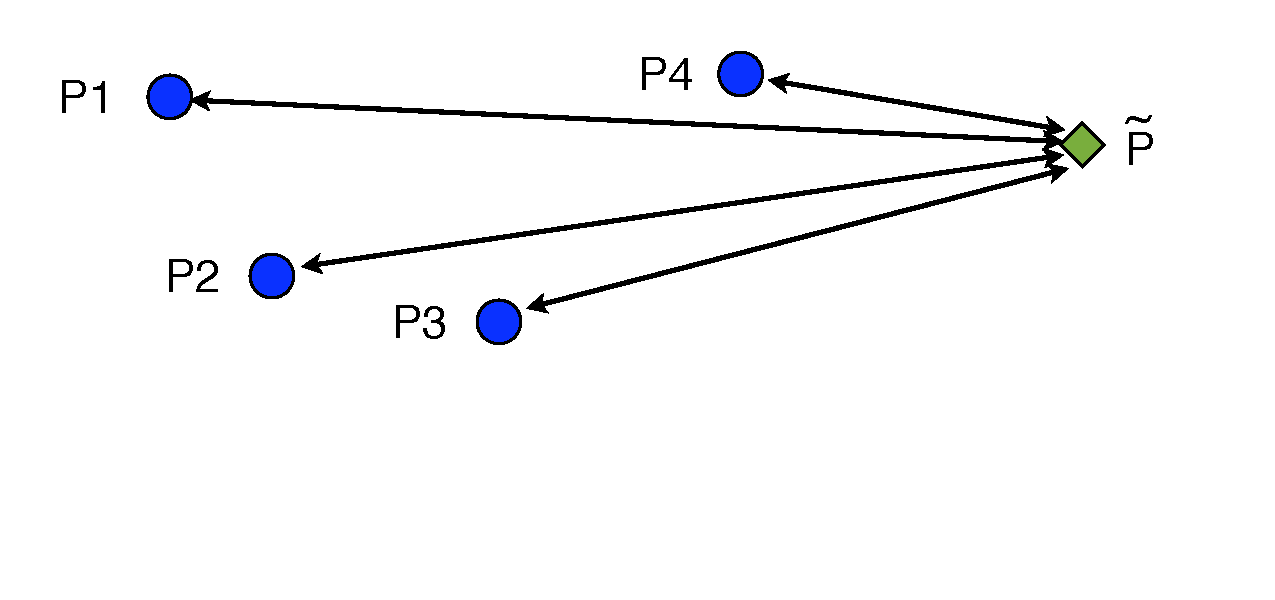
\includegraphics[width=10cm]{figures/divergenceAnalysis.pdf}
\end{frame}

% \iffalse
% \begin{frame}
% \frametitle{Proof of Lemma (1)}
% \R{\begin{eqnarray*}
% \lefteqn{
% \RE{\Pref}{\P_{t+1}} - \RE{\Pref}{\P_t}} \pause \\
% &=& 
% \sum_{i=1}^n \Pref(i) \ln {\Pref(i) \over \P_{t+1}(i)}
% - \sum_{i=1}^n \Pref(i) \ln {\Pref(i) \over \P_t(i)} \pause \\
% &=&
% \sum_{i=1}^n \Pref(i) \ln {\P_t(i) \over \P_{t+1}(i)}\pause \\
% &=&
% \sum_{i=1}^n \Pref(i) \ln {Z_t \over e^{\eta \M(i,\Qt)}}
% \end{eqnarray*}
% }
% \end{frame}


% \begin{frame}
% \frametitle{Proof of Lemma (2)}
% \R{\begin{eqnarray*}
% &=&
% \eta \sum_{i=1}^n \Pref(i) \M(i,\Qt) + \ln Z_t \pause \\
% &\leq&
% \eta \M(\Pref,\Qt)
% +
% \ln\brac{\sum_{i=1}^n \P_{t}(i) \left( 1- (1-e^{-\eta}) \M(i,\Qt) \right)}
% \pause
% \\
% &=&
% \eta \M(\Pref,\Q_t) 
% +
% \ln \left( 1-(1-e^{-\eta})\M(\Pt,\Qt) \right)
% \pause \\
% & \leq &
% \eta \M(\Pref,\Q_t)  + (1-e^{-\eta})\M(\Pt,\Qt)
% \end{eqnarray*}
% }
% \end{frame}
% \fi

\section{Proof of minmax theorem}

\begin{frame}
\frametitle{The minmax Theorem}
~\\
John von Neumann, 1928.
\\ ~ \\ \pause
\R{\[ \minp \maxq \mpq = \maxq \minp \mpq \]}
\\ ~ \\ \pause
In words: for \B{mixed} strategies, choosing second gives no advantage.
\end{frame}

\begin{frame}
\frametitle{Proving minmax Theorem using online learning (1)}
~\\
Row player chooses \R{$\P_t$} using learning alg. \\ \pause 
Column player chooses \R{$\Q_t$} \B{after row player} so that
\R{$\Qt = \arg \maxq \mptq$}
\\ \pause
Let \R{$\Pa \doteq \frac{1}{T} \sumt \Pt$} and
\R{$\Qa \doteq \frac{1}{T} \sumt \Qt$}
\\ \pause
\R{\em
\[
\begin{array}{rcll}
{\displaystyle{\minp \maxq \trans{\P}\M\Q}} 
 &\leq&
\displaystyle{\maxq \trans{\Pa}\M\Q} & \nextline
\pause
  &=&
\displaystyle{\maxq \frac{1}{T} \sumt \trans{\Pt}\M\Q}
                       &\mbox{\rm by definition of~~\Pa}\nextline
\pause
  &\leq&
\displaystyle{\frac{1}{T} \sumt \maxq \trans{\Pt}\M\Q} &
\end{array}
\]
}
\end{frame}


\begin{frame}
\frametitle{Proving minmax Theorem using online learning (2)}
\R{\em
\[
\begin{array}{rcll}
  &=&
\displaystyle{\frac{1}{T} \sumt \trans{\Pt}\M\Qt}
                       &\mbox{\rm by definition of~~\Qt}\nextline
\pause
  &\leq&
\displaystyle{\minp \frac{1}{T} \sumt \trans{\P}\M\Qt + \delt}
                       &\mbox{\rm by the Corollary} \nextline
\pause
  &=&
\displaystyle{\minp \trans{\P}\M\Qa + \delt}
                       &\mbox{\rm by definition of~~\Qa}\nextline
\pause
  &\leq&
\displaystyle{\maxq \minp \trans{\P}\M\Q + \delt.} &
\end{array}
\]
}
\pause
but \R{$\delt$} can be set arbitrarily small.
\end{frame}

% \iffalse
% \begin{frame}
% \frametitle{Minmax is weaker than diminishing regret}
% \begin{itemize}
% \item The minmax theorem proves the existence of an \B{Equilibrium}.
% \item Learning guarantees no regret with respect to the past.
% \item If all sides use learning, then game will converge to minmax equilibrium.
% \item If opponent is not optimally adversarial (limited by knowledge, computationa power...) then learning gives \B{better} performance than min-max.
% \item Is it realistic to assume that markets are at equilibrium?
% \item If game is not zero sum (allows incentives to collaborate) and all players
% use learning then game converges to \B{correlated equilibrium}.
% \end{itemize}
% \end{frame}
% \fi

%\iffalse %%%%%%%%%%%%%%%%%%%%%%%%%%%%%%%%%%%%%%%%%%%%%%%%%%%%%%%%%%%%%%%%%%

\section{Approximately solving games}

\begin{frame}
  \frametitle{Solving a game}
  \begin{itemize}
    \item to \B{solve} a game is to find the min-max mixed strategies
      \R{$\P,\Q$}
    \item Suppose that \ouralg is playing \R{$\P_1,\P_2,$} against a
      worst case adversary that playes second: 
      adversary that plays \R{$\Q_1,\Q_2,\ldots$} such that \R{$\Qt =
        \arg \maxq \mptq$}.
    \item Without loss of generality \R{$\Qt$} is a pure strategy
      (prob. 1 on a single action).
     \item Let \R{$\Pa \doteq \frac{1}{T} \sumt \Pt$}, \R{$\Qa \doteq \frac{1}{T} \sumt \Qt$}
  \end{itemize}
\end{frame}

\subsection{Fixed Learning rate}
\begin{frame}
\frametitle{Using average distributions}
\begin{itemize}
\item Von Neumann Min/Max Thm: \R{$ v \doteq \minp \maxq \mpq = \maxq \minp \mpq $}
\item Fixing \R{$T$} and letting \R{$ \eta = \ln \paren{ 1+\sqrt{\frac{2\ln n}{T}} }$}
\item Two immediate corrolaries of the proof of the min/max Thm:
\R{ \[    \maxq \M(\Pa,\Q) \leq v + \delt.
          \minp \M(\P,\Qa) \geq v - \delt \]}

\end{itemize}
\end{frame}

\subsection{Variable learning rate}
\begin{frame}
\frametitle{Using the final row distribution \R{\lwalgvar}}
\begin{itemize}
\item Can we make the row distribution converge?
\item Suppose we have an upper bound on the value of the game \R{$u
  \geq v$}
\item {\bf Good Enough:} If \R{$\M(\Pt,\Qt) \leq u$} the row player does nothing
\R{$\P_{t+1}=\P_t$}
\item {\bf Learn:} If \R{$\M(\Pt,\Qt) > u$} set
  \R{$$
     \eta= \ln { (1-u) \M(\Pt,\Qt) \over u (1 - \M(\Pt,\Qt))}~.
    $$}
\end{itemize}
\end{frame}

\begin{frame}
\frametitle{Bound for \R{\lwalgvar}}
\begin{itemize}
\item Let \R{$\Pref$} be any mixed strategy for the rows such that 
\R{$\maxq \M(\Pref,\Q) \leq u$}
\item
  Then on any iteration of algorithm \R{\lwalgvar} in which 
\R{$\M(\Pt,\Qt) \geq u$} the relative entropy between \R{$\Pref$} and \R{$\P_{t+1}$}
satisfies
\R{\[
\RE{\Pref}{\P_{t+1}} \leq \RE{\Pref}{\Pt} - \RE{u}{\M(\Pt,\Qt)}~.
\]}
\end{itemize}
\end{frame}

\iffalse %%%%%%%%%%%%%%%%%%%%%%%%%%%%%%%%%%%%%%%%%%%%%%%%%%%%%%%%%%%%%%%%%%
\fi %%%%%%%%%%%%%%%%%%%%%%%%%%%%%%%%%%

\end{document}


